\documentclass[../fractal_dimensions_quasicrystals.tex]{subfiles}
\begin{document}


    	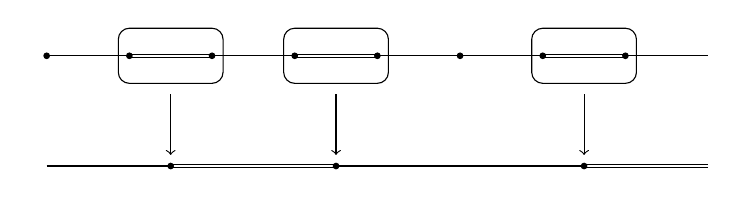
\begin{tikzpicture}[scale=.7]
    		\newcommand{\orig}{-1.5}
    		\newcommand{\trans}{1.5}
    		\newcommand{\vertspac}{-2.}
    		\newcommand{\vertsize}{.5} % vertical spand of the rectangles
    		\newcommand{\del}{.2}
    	
    		% initial chain
    	
    		% bonds 
        	\draw[-] (\orig, 0)  node [left] {}  -- (\orig+\trans, 0);
			\draw[-,double] (\orig+\trans,0) -- (\orig+2*\trans,0); % node [midway, above] {$t_s$};
			\draw[-] (\orig+2*\trans,0) -- (\orig+3*\trans,0); % node [midway, above] {$t_w$};	
			\draw[-,double] (\orig+3*\trans,0) -- (\orig+4*\trans,0); % node [midway, above] {$t_s$};
			\draw[-] (\orig+4*\trans,0) -- (\orig+5*\trans,0); % node [midway, above] {$t_w$};
			\draw[-] (\orig+5*\trans,0) -- (\orig+6*\trans,0); % node [midway, above] {$t_w$};
			\draw[-,double] (\orig+6*\trans,0) -- (\orig+7*\trans,0); % node [midway, above] {$t_s$};
			\draw[-] (\orig+7*\trans,0) -- (\orig+8*\trans,0); % node [midway, above] {$t_w$};
    	
    		% sites
			\foreach \x in {0,...,7}
		      \filldraw (\orig+\x*\trans,0) circle (0.05); % node [below] {$\ket{\x}$};
		      
		    % rectangles around molecules
		    \draw [rounded corners] (\orig +\trans-\del,-\vertsize) rectangle (\orig+2*\trans+\del,\vertsize);
		    \draw [rounded corners] (\orig +3*\trans-\del,-\vertsize) rectangle (\orig+4*\trans+\del,\vertsize);
		    \draw [rounded corners] (\orig +6*\trans-\del,-\vertsize) rectangle (\orig+7*\trans+\del,\vertsize);
		    
		    % arrows below rectangles
		    \draw [->] (\orig+1.5*\trans,-\vertsize-\del) -- (\orig+1.5*\trans,\vertspac+\del);
		    \draw [->] (\orig+3.5*\trans,-\vertsize-\del) -- (\orig+3.5*\trans,\vertspac+\del);
		    \draw [->] (\orig+6.5*\trans,-\vertsize-\del) -- (\orig+6.5*\trans,\vertspac+\del);
		      
			% molecular chains
			
			\foreach \x in {1}
			{
				\draw[-] (\orig, \x*\vertspac) node [left] {} -- (\orig+1.5*\trans, \x*\vertspac);
				\draw[-,double] (\orig+1.5*\trans, \x*\vertspac) -- (\orig+3.5*\trans, \x*\vertspac);
				\draw[-] (\orig+3.5*\trans, \x*\vertspac) -- (\orig+6.5*\trans, \x*\vertspac);
				\draw[-,double] (\orig+6.5*\trans, \x*\vertspac) -- (\orig+8*\trans, \x*\vertspac);
				
				\filldraw (\orig+1.5*\trans,\x*\vertspac) circle (0.05);
				\filldraw (\orig+3.5*\trans,\x*\vertspac) circle (0.05);
				\filldraw (\orig+6.5*\trans,\x*\vertspac) circle (0.05);
			}
		\end{tikzpicture}

\end{document}